\section*{Solutions}


\begin{figure}[H]
\centering
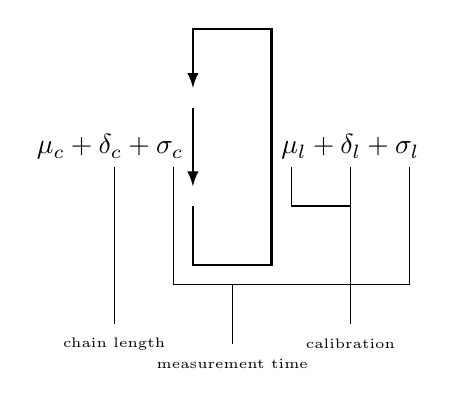
\begin{tikzpicture}

\draw [>=latex,->, line width = 0.3mm]
(0,1.25) |-
(1,0.5) --
(1,3.5) -|
(0,2.75);

\draw [>=latex,->, line width = 0.3mm]
(0,2.5) --
(0,1.5);

\node [anchor=west] at (1,2) {$\mu_l+\delta_{l}+\sigma_{l}$};
\node [anchor=east] at (0,2) {$\mu_c+\delta_{c}+\sigma_{c}$};

% measurement time
\draw (-0.25,1.75) -- (-0.25,0.25) -|  (0.5,-0.5);
\draw (0.5,0.25) -| (2.75,1.75);
\node at (0.5,-0.75) {\tiny{measurement time}};

% callibration
\draw (2,-0.25) -- (2,1.75);
\draw (1.25,1.75) |- (2,1.25);
\node at (2,-0.5) {\tiny{calibration}};

% chain length
\draw (-1,-0.25) -- (-1,1.75);

\node at (-1,-0.5) {\tiny{chain length}};
\end{tikzpicture}
\caption{math}
\label{tkz:math}
\end{figure}


\begin{align*}
\sigma_{tot} = \sqrt{\frac{\sigma_{c,s}^2}{\text{components}}+\frac{\sigma_{c,d}^2+\sigma_{l,d}^2}{\text{counts}}}
\end{align*}

\begin{align*}
LSB &= \frac{T}{\text{counts}}\\
t_{meas} &= T\cdot \text{counts} = \frac{T^2}{LSB}\\
bits &= \lceil\log_2(\text{counts})\rceil
\end{align*}
%For example, take a path with 50 components of $\approx 50\,ps$ delay, with a requirement of $1\,ps$ resolution
\begin{align*}
\text{for 50 components with $\approx 50\,ps$} &\text{ delay, and $1\,ps$ resolution requirement}  \\
T &= 2500\,ps\\
\text{counts} &= 2500\\
t_{meas} &= 6.25\,\mu s\\
bits &= 12
\end{align*}

\begin{align*}
\text{for 10 components with $\approx 50\,ps$} &\text{ delay, and $1\,ps$ resolution requirement}  \\
T &= 500\,ps\\
\text{counts} &= 500\\
t_{meas} &= 250\,ns\\
bits &= 9
\end{align*}

